% Finite Precision Loop Mechanics: A Mechanism-First Note
% Author: Jakob Reinehr
% Date: May 2026
% Broader theory note accompanying the narrow numerical preprint.

\documentclass[11pt,a4paper]{article}
\usepackage[utf8]{inputenc}
\usepackage[T1]{fontenc}
\usepackage[scaled=0.92]{helvet}
\renewcommand\familydefault{\sfdefault}
\usepackage{amsmath,amssymb}
\usepackage{booktabs}
\usepackage{graphicx}
\usepackage{hyperref}
\usepackage{geometry}
\geometry{margin=2.5cm}
\graphicspath{{../figures/}}

\hypersetup{
  colorlinks=true,
  linkcolor=black,
  citecolor=black,
  urlcolor=blue
}

\newcommand{\ZGi}{\mathbb{Z}[i]}
\newcommand{\modp}{\ZGi/(p)}

\newcommand{\schematic}[1]{%
\begin{center}
\fbox{%
\begin{minipage}{0.92\linewidth}
\centering
#1
\end{minipage}}
\end{center}
}

\title{Finite Precision Loop Mechanics:\\A Mechanism-First Note}
\author{Jakob Reinehr}
\date{May 2026}

\begin{document}
\maketitle

\begin{abstract}
This note presents the mechanism-first idea behind finite-precision loop
mechanics. The starting suspicion is conservative: no physical system can
instantiate infinitely many exact digits. If physical evolution has finite
distinguishability, then rounding, thresholding, overflow, or some related
finite-resolution process is not merely an error in our description. It may
be a source of physical structure. In a finite state space, recurrent cycles
and attractor basins are structurally expected. The proposal explored here is
that some stable or metastable attractor cycles may behave like matter-like
objects, while linear untrapped processes are light-like. This broader
mechanism note is intentionally distinct from the narrower numerical
preprint: the numerical evidence is reproducible and concrete; the physical
interpretation is a candidate mechanism to be tested.
\end{abstract}

\tableofcontents
\newpage

%------------------------------------------------------------------------------
\section{Purpose and Status}
%------------------------------------------------------------------------------

This document is a synthesis of the theory fragments in the repository. It is
not the same thing as the numerical preprint. The preprint is deliberately
narrow: attractor periods in finite Gaussian-integer systems show close
coincidences with several Standard-Model mass ratios, together with a
split/inert prime control. This note asks a different question:

\begin{quote}
If finite attractor cycles were physically relevant, what kind of mechanics
would they suggest?
\end{quote}

The answer is speculative. The goal is not to claim a derivation of the
Standard Model, quantum field theory, gravity, Lorentz invariance, gauge
symmetry, or the fine-structure constant. The goal is to organize the
mechanism clearly enough that it can be criticized, simulated, falsified, or
improved.

Throughout the note, there are three levels of claim:

\begin{enumerate}
\item \textbf{Mechanism:} finite precision creates thresholds, residues,
attractor basins, and loop traps.
\item \textbf{Toy model evidence:} finite systems on $\modp$ produce
structured period spectra and mass-ratio coincidences.
\item \textbf{Physical interpretation:} some loop traps might correspond to
matter-like processes; linear untrapped processes might correspond to
light-like propagation.
\end{enumerate}

Only the second level is currently concrete and reproducible. The first level
is a general mechanistic argument. The third level is the physical hypothesis.

%------------------------------------------------------------------------------
\section{The Starting Suspicion: Finite Actual Precision}
%------------------------------------------------------------------------------

The starting point is weaker than saying that the universe is a digital
computer. It is simply this:

\schematic{
\textbf{No actual physical system should require infinitely many exact digits
to exist.}
}

Continuous mathematics is extraordinarily successful, but it may be an
effective language rather than an ontology. A real physical state must be
physically instantiated. If a difference can never be stored, transmitted,
distinguished, or acted upon, then treating that difference as an actual
physical distinction may be an over-idealization.

Several motivations point in this direction:

\begin{itemize}
\item finite regions appear to have finite information capacity;
\item measurement never accesses infinitely many digits;
\item chaotic dynamics makes infinite precision physically consequential in a
way no finite system can maintain;
\item quantum theory already limits simultaneous distinguishability;
\item gravitational and information bounds suggest that arbitrary information
density is not physical.
\end{itemize}

The claim is not that continuum mathematics is wrong. The claim is that it may
describe the large-scale limit of a finite-precision process.

%------------------------------------------------------------------------------
\section{Rounding as Mechanism}
%------------------------------------------------------------------------------

In numerical computation, rounding is usually treated as an implementation
defect. In this mechanism, finite resolution is promoted to a possible source
of physical structure.

Rounding should be understood broadly. It need not mean downward truncation.
It can mean any map in which many nearby possible values become one effective
state:

\schematic{
\[
\text{many nearby states}
\quad \longrightarrow \quad
\text{one effective state}
\]
}

That creates:

\begin{itemize}
\item equivalence classes;
\item thresholds;
\item basins of attraction;
\item ignored weak inputs;
\item sudden transitions when a threshold is crossed.
\end{itemize}

These are exactly the ingredients needed for stability, inertia-like
resistance, and effective interaction ranges.

The finite models in this repository use modular arithmetic over Gaussian
integers:

\[
\modp.
\]

This is not claimed to be the final physical cut-off. It is a minimal finite
test bed. It is useful because $\ZGi$ is the smallest integer-like structure
with two orthogonal components. Multiplication by $i$ rotates by $90^\circ$,
so phase-like behavior appears arithmetically rather than as an added
continuous variable.

%------------------------------------------------------------------------------
\section{Recurrence and Loop Traps}
%------------------------------------------------------------------------------

A deterministic system with finitely many states cannot keep producing new
states forever. If a trajectory is followed long enough, it must either fail
to converge within the observation window or revisit a previous state. Once a
state is revisited, the future repeats.

\schematic{
\[
x_t = x_s
\quad \Longrightarrow \quad
x_{t+1}=x_{s+1}
\quad \Longrightarrow \quad
x_{t+2}=x_{s+2}
\quad \Longrightarrow \quad \cdots
\]
}

This creates a cycle. A \emph{loop trap} is a stable or metastable cycle in
finite process space. It is important that ``loop'' does not primarily mean a
literal circle in background space. It means recurrence in state space:

\[
A \longrightarrow B \longrightarrow C \longrightarrow A.
\]

Finite precision makes such cycles more physically plausible because almost
closed returns can become exact effective returns:

\schematic{
\[
\text{almost } A
\quad \xrightarrow{\text{finite precision}}
\quad A
\quad \xrightarrow{\text{cycle continues}}
\quad B
\]
}

In a continuous system, tiny mismatches can prevent closure forever. In a
finite-precision system, a rounding basin can turn approximate recurrence into
actual recurrence. This is the basic reason rounding is treated as a kind of
``glue'' for loop traps.

%------------------------------------------------------------------------------
\section{Light-Like and Matter-Like Modes}
%------------------------------------------------------------------------------

The simplest process in this framework is not matter. It is light-like
propagation. A minimal linear step is:

\[
z_{\mathrm{out}} = w z_{\mathrm{in}} \pmod p.
\]

There is one input, one output, and no local self-reference. A pure phase
rotation such as $w=i$ requires no amplitude growth and little or no rounding
in the idealized step.

Matter-like behavior begins when a process no longer remains a simple linear
chain. It acquires multiple inputs, local self-processing, self-coupling, and
rounding-dominated closure.

\begin{figure}[htbp]
\centering
\fbox{\begin{minipage}{0.9\linewidth}
\centering
\begin{tabular}{ccc}
\textbf{Linear process} && \textbf{Loop trap}\\[0.4em]
$z_{\mathrm{in}} \to w z_{\mathrm{in}} \to z_{\mathrm{out}}$
&&
$A \to B \to C \to A$\\[0.4em]
one input / one output && self-referential cycle\\
untrapped && attractor basin\\
light-like && matter-like
\end{tabular}
\end{minipage}}
\caption{The core distinction is operational. A light-like process is linear
and untrapped. A matter-like process is closed into a stable or metastable
attractor cycle.}
\label{fig:linear_vs_loop}
\end{figure}

Thus matter is not a second substance. It is the same kind of process in a
closed, self-referential mode:

\[
\text{light} = \text{process that propagates},
\qquad
\text{matter} = \text{process that gets caught in itself}.
\]

%------------------------------------------------------------------------------
\section{The Schmalznudel Mechanism}
%------------------------------------------------------------------------------

The numerical mass-ratio results show that finite Gaussian-ring systems can
generate nontrivial attractor spectra. But numbers alone do not explain why a
loop would behave like a particle. The Schmalznudel mechanism is the proposed
physical interpretation layer.

In its minimal form, a Schmalznudel is a small, strongly coupled loop with
self-reference. A toy update rule is:

\[
z_j(t+1)
=
z_j(t)^2
+
\sum_k w_{jk} z_k(t)
\pmod n.
\]

The ingredients are:

\begin{itemize}
\item $\ZGi$ gives two orthogonal components, analogous to field quadratures;
\item linear transport is the light-like part;
\item the local $z^2$ term is nonlinear self-reference;
\item self-coupling is a minimal memory or mass-like term;
\item modular rounding creates the finite basin that lets a loop close.
\end{itemize}

The short version is:

\schematic{
\begin{tabular}{rcl}
linear process & $\longrightarrow$ & light-like propagation\\
closed loop process & $\longrightarrow$ & matter-like attractor\\
rounding threshold & $\longrightarrow$ & inertia and stability\\
rounding residue & $\longrightarrow$ & radiation, decay, vacuum-like noise\\
potential pressure & $\longrightarrow$ & repulsion and relational space
\end{tabular}
}

This layer is not established physics. It is a mechanistic hypothesis to be
tested after the numerical core has survived criticism.

%------------------------------------------------------------------------------
\section{Inertia from Rounding}
%------------------------------------------------------------------------------

Inertia is usually treated as a primitive property of mass. In this mechanism,
it is interpreted as loop stability under finite precision:

\schematic{
\textbf{Inertia is the cost of forcing a stable loop to leave its preferred
attractor continuation.}
}

Two mechanisms are proposed.

\paragraph{Threshold effect.}
Finite precision creates a basin around an attractor. If a perturbation is
smaller than the relevant threshold, then:

\[
\text{state}+\text{perturbation}
\quad \longrightarrow \quad
\text{same rounded successor}.
\]

From outside, this looks like resistance: input was applied, but no effective
state change is observed.

\paragraph{Internal dominance.}
A loop trap is not a passive stored value. Each update combines local
self-processing, neighboring inputs, self-coupling, and rounding. An external
input is only one contribution to a process already dominated by internal
terms. Unless it changes the rounded successor, it is absorbed by the
attractor.

This suggests candidate mass-like measures:

\begin{itemize}
\item basin size;
\item return probability after perturbation;
\item minimum perturbation needed to change attractor;
\item internal operation density;
\item period and frequency structure.
\end{itemize}

The current numerical work uses periods and period ratios. A stronger theory
would connect those ratios to perturbation resistance and basin geometry.

%------------------------------------------------------------------------------
\section{Residues, Radiation, and Decay}
%------------------------------------------------------------------------------

Finite precision creates a question that modular simulations often hide: what
happens to the part of the update that does not fit into the finite register?
For a loop node, write the unmodded intermediate value as:

\[
S_j = z_j(t)^2 + \sum_k w_{jk}z_k(t).
\]

The finite update keeps:

\[
z_j(t+1)=S_j \bmod p.
\]

The discarded part is the residue:

\[
R_j = S_j - (S_j \bmod p).
\]

\begin{figure}[htbp]
\centering
\fbox{\begin{minipage}{0.9\linewidth}
\centering
\[
\underbrace{S_j}_{\text{unmodded update}}
\quad \longrightarrow \quad
\underbrace{S_j \bmod p}_{\text{kept finite state}}
\quad + \quad
\underbrace{R_j}_{\text{residue}}
\]
\vspace{0.3em}
\begin{tabular}{rl}
stable loop: & residues cancel or are reabsorbed over a full period\\
perturbed loop: & residues fail to cancel and may leave as linear output\\
metastable loop: & threshold crossing may trigger transition or decay
\end{tabular}
\end{minipage}}
\caption{Residue accounting is the proposed bridge from finite precision to
radiation-like leakage, decay, and vacuum-like fluctuation. In current toy
simulations the residue is discarded; in a physical mechanism it must be
accounted for.}
\label{fig:residue_schematic}
\end{figure}

In the simplest simulation, the residue is thrown away. Physically, that
cannot be the final story if potential or energy is to be conserved. The
candidate interpretations are:

\begin{itemize}
\item a stable loop has balanced net residue over a full period, so it does
not radiate in its unperturbed state;
\item a perturbed loop produces non-canceling residue, which leaves as a
linear process;
\item short-lived residue imbalances appear as vacuum-like fluctuations;
\item persistent residue transfer changes effective coupling strengths.
\end{itemize}

This gives a candidate mechanism for radiation and decay without adding a
separate process. The same finite rounding that stabilizes loops can also
destabilize them near basin boundaries.

%------------------------------------------------------------------------------
\section{Interactions as Loop Exchange Modes}
%------------------------------------------------------------------------------

In this mechanism, an interaction is not a primitive force added to matter. It
is a mode of process exchange between loop traps:

\[
\text{stable loops}
\quad \longleftrightarrow \quad
\text{shared inputs, residues, asymmetries, coupling deformation}.
\]

Different interaction-like behaviors correspond to different ways loops can
affect one another.

\begin{table}[htbp]
\centering
\caption{Qualitative interaction hierarchy suggested by the loop mechanism.}
\begin{tabular}{lll}
\toprule
Mode & Candidate mechanism & Expected range\\
\midrule
Electromagnetic-like & loop asymmetry emits/absorbs linear residue & long\\
Strong-like & sub-loops only close as a composite attractor & short\\
Weak-like & loop-type transformation through massive loop mediator & very short\\
Gravity-like & statistical bias of loop fluctuations on relations & long, weak\\
\bottomrule
\end{tabular}
\label{tab:interaction_hierarchy}
\end{table}

The goal is not to force the Standard Model into the mechanism by analogy. The
goal is to identify testable process signatures for each interaction type. For
example, the strong-like interpretation becomes meaningful only if isolated
sub-loops fail where composite sub-loop systems close reliably, and if
attempted separation creates rearranged composites rather than free sub-loops.

%------------------------------------------------------------------------------
\section{Emergent Relational Space}
%------------------------------------------------------------------------------

This mechanism does not begin with space as a container. It begins with
processes, relations, coupling strengths, and potential gradients.

\schematic{
\begin{tabular}{ccc}
\text{primitive statement} &&
\text{emergent spatial rendering}\\[0.4em]
process $A$ influences process $B$ with strength $w$
&&
object $A$ is near object $B$
\end{tabular}
}

Space is interpreted as the large-scale ordering of stable relations between
loop traps. A loop trap is internally process-like, not spatial in the ordinary
sense. Space emerges between stable loops:

\[
\text{loop }A
\quad \longleftrightarrow \quad
\text{relation structure}
\quad \longleftrightarrow \quad
\text{loop }B.
\]

The proposed reason for three effective dimensions combines two pressures:

\begin{enumerate}
\item potential must be able to disperse;
\item stable structures must remain possible.
\end{enumerate}

In one and two dimensions, random walks are recurrent: they return with
probability one. Potential has difficulty escaping its origin cleanly. In
three dimensions, random walks become transient: potential can disperse. In
four or more dimensions, dispersion is easier, but stable knot-like or
bound-loop structures become less natural.

The conjecture is therefore:

\schematic{
\[
\text{3D}
=
\text{lowest dimension that permits robust dispersion}
=
\text{highest dimension that preserves stable knot-like closure}.
\]
}

This is not yet a result. It is a testable mechanistic bridge between loop
stability and emergent relational geometry.

%------------------------------------------------------------------------------
\section{Numerical Evidence Summary}
%------------------------------------------------------------------------------

The broader mechanism would be thin without concrete evidence that small
finite systems can produce structured spectra. The current evidence is
narrower than the mechanism:

\begin{itemize}
\item $\modp$ attractor spectra are nontrivial;
\item $p=13$, $k=6$, and weights $(1,i)/(i,1)$ give close lepton-ratio
coincidences;
\item split primes and inert primes differ sharply in tested symmetric scans;
\item coupled sub-loops produce quark-ratio coincidences;
\item degree $d=2$ maximizes attractor entropy among tested polynomial degrees.
\end{itemize}

\begin{figure}[htbp]
\centering
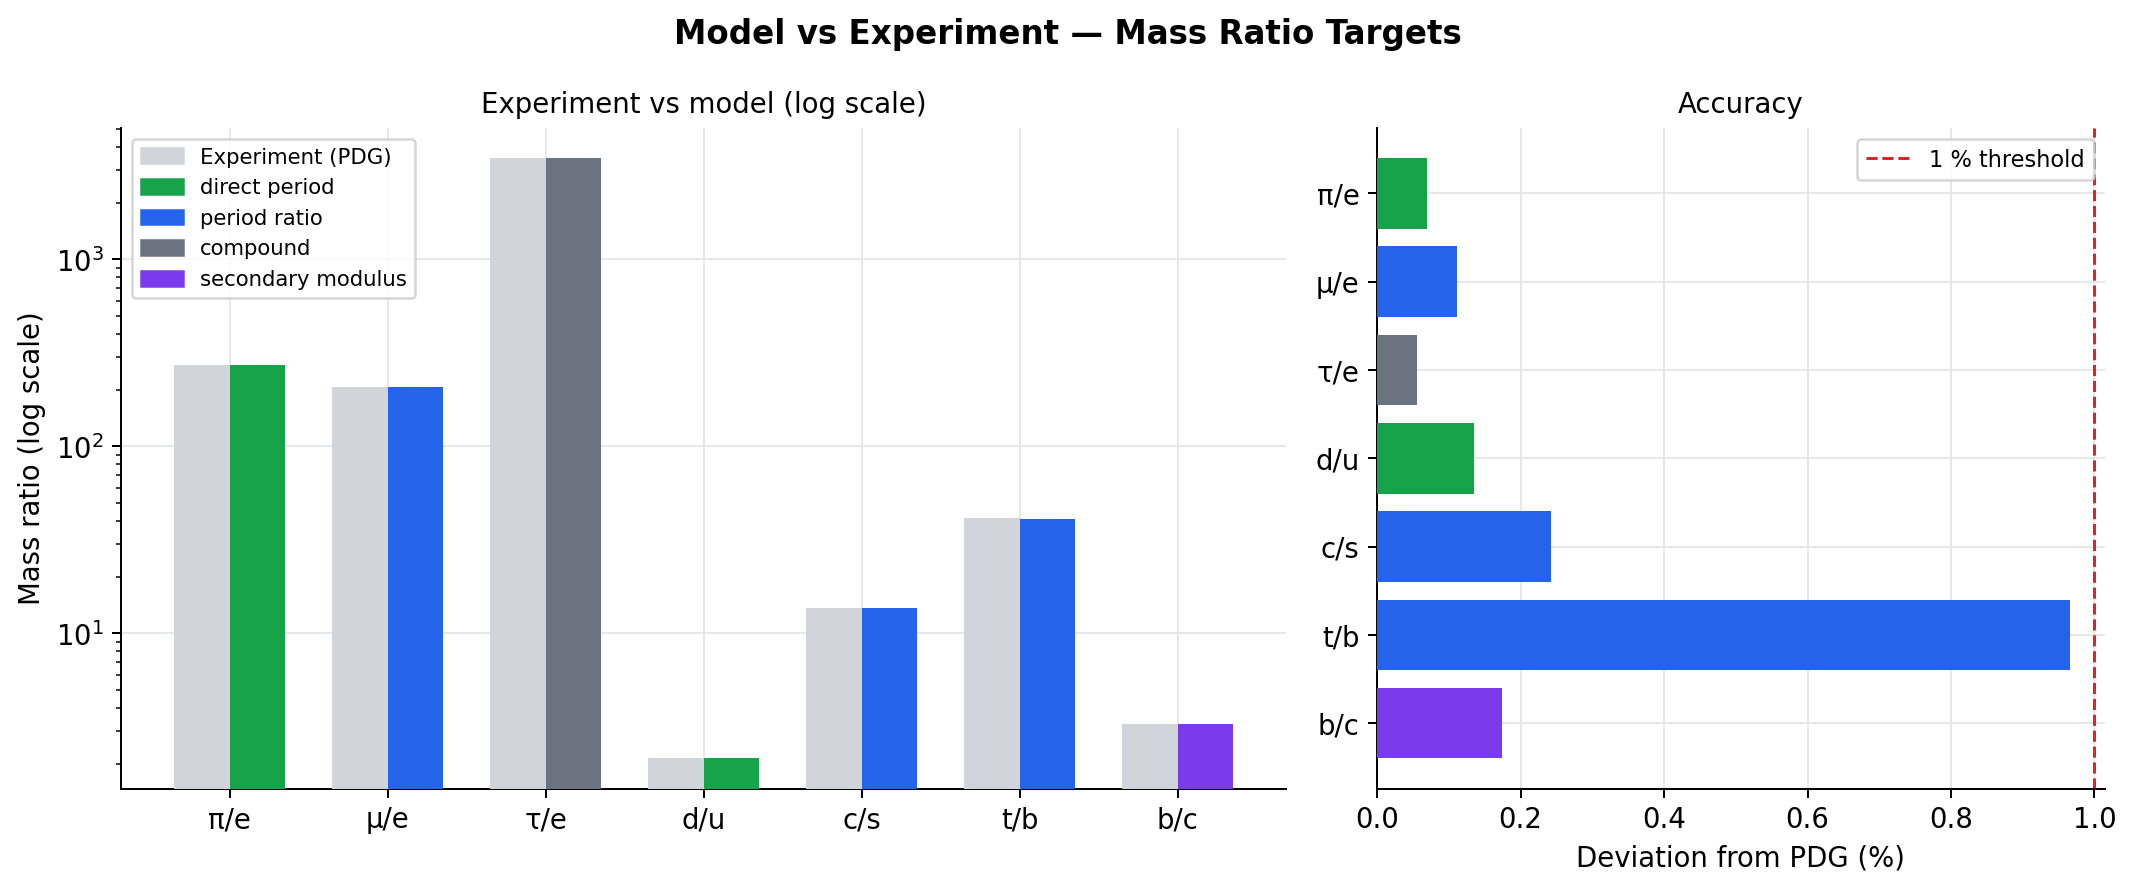
\includegraphics[width=\textwidth]{fig1_mass_ratios.png}
\caption{Model vs experiment for seven mass-ratio targets. This figure
belongs to the numerical observation, not to the speculative mechanism by
itself.}
\label{fig:note_mass_ratios}
\end{figure}

\begin{figure}[htbp]
\centering
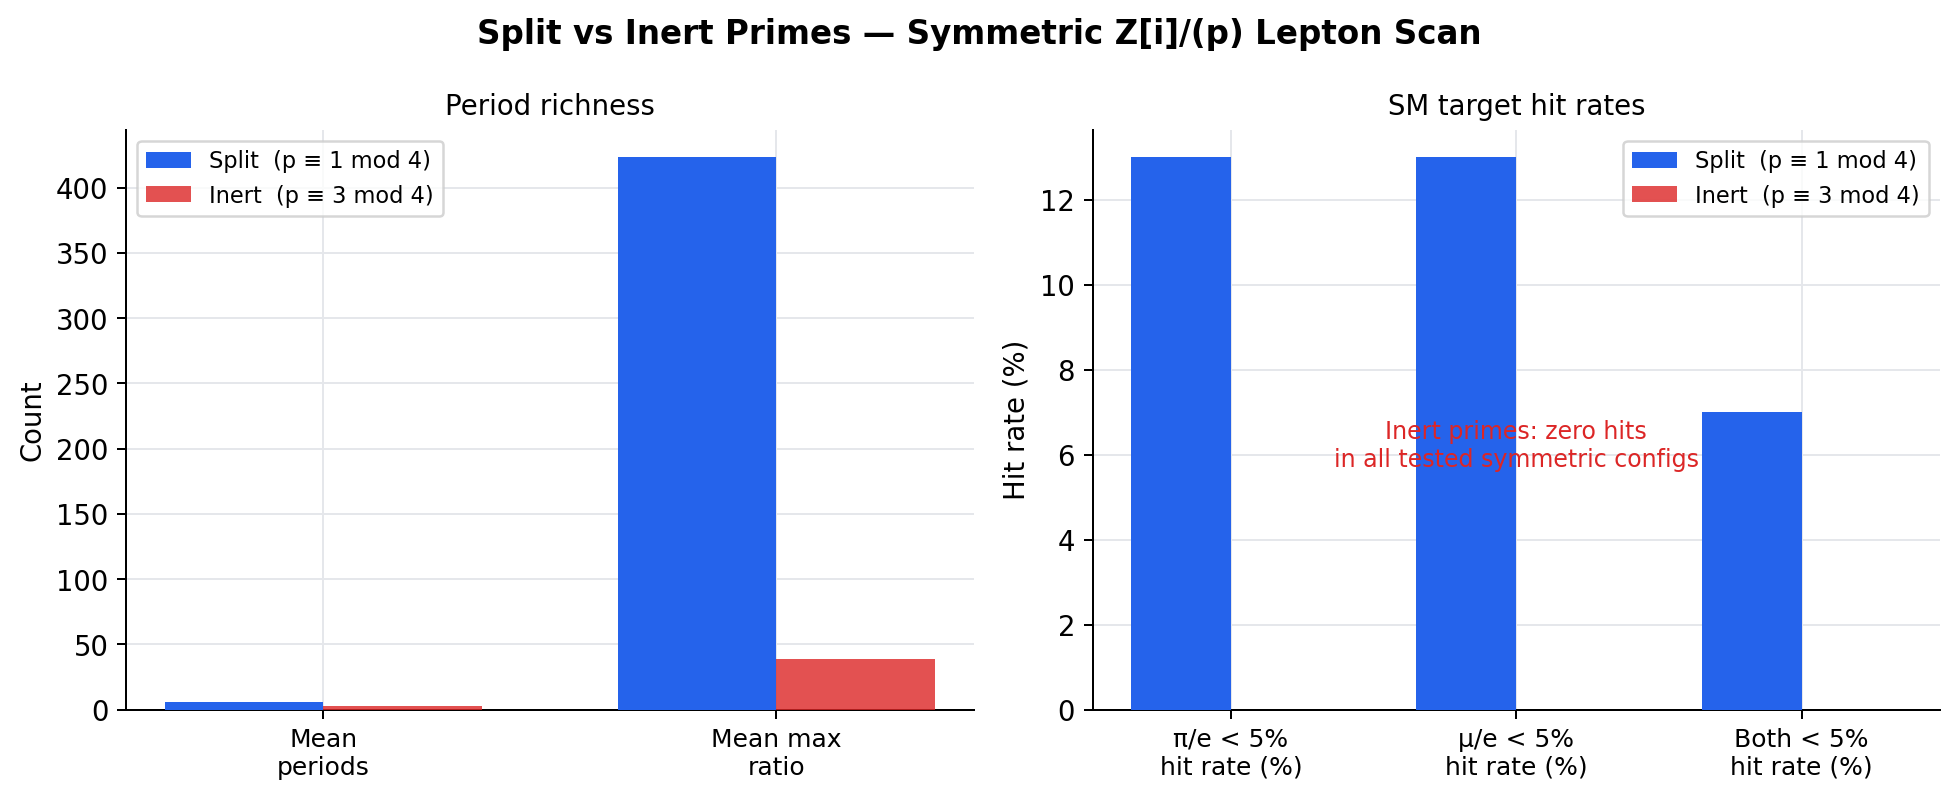
\includegraphics[width=\textwidth]{fig2_split_inert.png}
\caption{Split vs inert prime comparison in the symmetric $\modp$ lepton scan.
The split/inert distinction is the strongest structural control currently
available in the evidence package.}
\label{fig:note_split_inert}
\end{figure}

\begin{figure}[htbp]
\centering
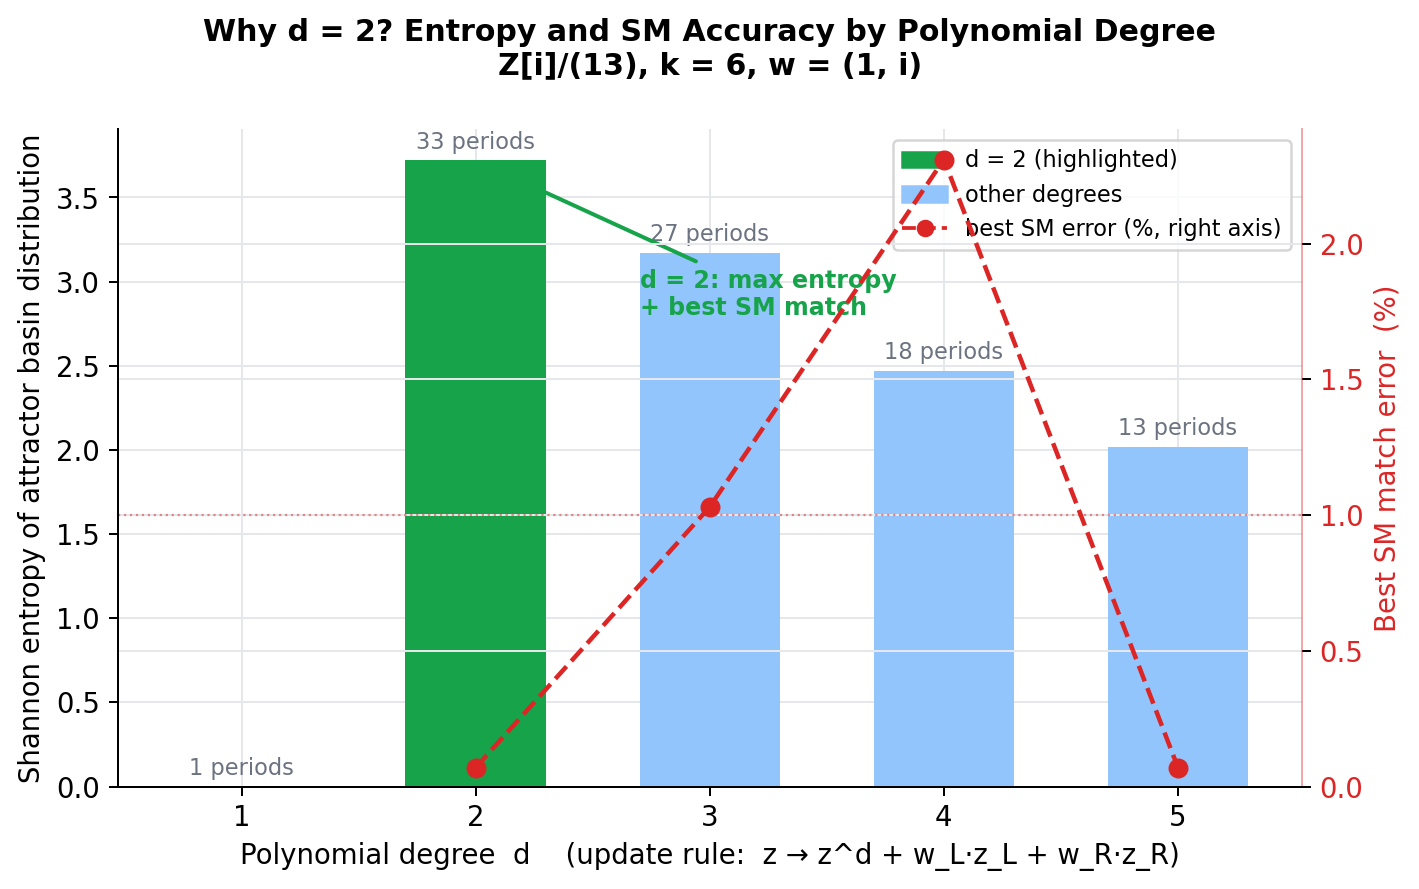
\includegraphics[width=0.86\textwidth]{fig3_entropy_degree.png}
\caption{Entropy and Standard-Model target accuracy by polynomial degree.
Within the tested setup, $d=2$ both maximizes attractor richness and gives the
closest simultaneous lepton-ratio hits.}
\label{fig:note_entropy_degree}
\end{figure}

These figures do not prove the physical interpretation. They justify taking
the finite loop-trap mechanism seriously enough to test it.

%------------------------------------------------------------------------------
\section{Predictions and Tests}
%------------------------------------------------------------------------------

The mechanism should not remain only a story. It must produce tests that can
fail. The near-term tests are computational.

\subsection{Residue balance}

\textbf{Claim:} stable unperturbed loops should have balanced net residue over
a full period.

\textbf{Test:}

\begin{enumerate}
\item For each attractor, compute the unmodded intermediate sum $S_j$.
\item Compute $R_j=S_j-(S_j \bmod p)$.
\item Sum residues across nodes and across one full period.
\item Compare stable, metastable, and unstable attractors.
\end{enumerate}

\textbf{Possible falsification:} stable attractors show arbitrary
non-canceling residue with no structure.

\subsection{Perturbed residue emission}

\textbf{Claim:} perturbations should create non-canceling residue before
transition or decay.

\textbf{Test:}

\begin{enumerate}
\item Start on a known attractor.
\item Apply controlled perturbations of increasing size.
\item Measure return, transition, escape, and residue imbalance.
\item Check whether residue imbalance predicts escape.
\end{enumerate}

\subsection{Inertia proxy}

\textbf{Claim:} mass-like resistance should correlate with basin geometry and
return rates.

Candidate measures include period, basin size, return probability after
perturbation, minimum perturbation that changes the attractor, and residue
imbalance under perturbation. The theory becomes stronger if these quantities
form a coherent hierarchy.

\subsection{Interaction sectors and sub-loop confinement}

Future tests should classify attractors by chirality, phase rotation, residue
pattern, and coupling asymmetry. Coupled pairs of attractors should then be
tested for attraction, repulsion, transition, or composite closure. The
strong-like sub-loop claim is weakened if isolated sub-loops close just as
well as composite sub-loop systems.

\subsection{Emergent dimension}

The 3D conjecture needs simulation. A useful test would build adaptive
relational graphs with finite capacity and potential pressure, allow residue
or pressure to modify couplings, then estimate effective graph dimension. The
mechanism is weakened if no tendency toward stable effective dimension appears.

%------------------------------------------------------------------------------
\section{Limitations}
%------------------------------------------------------------------------------

This note should be read with explicit limits.

\begin{itemize}
\item It does not derive the Standard Model.
\item It does not derive gauge symmetry in its established mathematical form.
\item It does not derive Lorentz invariance or scattering amplitudes.
\item It does not provide a quantum field theory.
\item It does not derive gravity.
\item It does not derive the fine-structure constant.
\item It does not prove that physical states are literally elements of
$\modp$.
\item It does not remove the search-space caveat from the historical numerical
exploration.
\end{itemize}

The mechanism would be damaged if residue accounting shows no conservation-like
structure, if perturbation resistance fails to correlate with any mass-like
proxy, if split/inert differences vanish under cleaner replication, or if
period-ratio hits disappear under stricter pre-registered target lists.

A mechanism that cannot be broken cannot become physics.

%------------------------------------------------------------------------------
\section{Conclusion}
%------------------------------------------------------------------------------

Finite-precision loop mechanics begins with a modest suspicion: exact
real-valued physical states may be an idealization. Once finite precision is
taken seriously, rounding is no longer merely error. It can create thresholds,
basins, residues, and stable cycles. Some cycles may behave as matter-like
loop traps; linear untrapped processes may behave as light-like propagation.

The numerical evidence on $\modp$ does not establish the full physical
interpretation. It does, however, show that small finite phase-like systems can
produce rich attractor spectra, sharp split/inert differences, and surprising
mass-ratio coincidences. That is enough to motivate the next step: residue,
perturbation, basin, and relational-space tests that can fail.

%------------------------------------------------------------------------------
\begin{thebibliography}{9}
%------------------------------------------------------------------------------

\bibitem{koide1983}
Y.~Koide,
\textit{A fermion-boson composite model of quarks and leptons},
Phys.\ Lett.\ B \textbf{120}, 161--165 (1983).
\url{https://doi.org/10.1016/0370-2693(83)90644-5}

\bibitem{thooft2014}
G.~'t~Hooft,
\textit{The Cellular Automaton Interpretation of Quantum Mechanics},
arXiv:1405.1548 (2014); Springer 2016.
\url{https://doi.org/10.1007/978-3-319-41285-6}

\bibitem{cambridge2025}
[Author(s) not listed in open-access record],
\textit{The Discrete Algebraic Structure of the Fermion Mass Spectrum
and its Pythagorean Geometric Origin},
Cambridge Open Engage, 29 December 2025 (preprint, not peer-reviewed).
\url{https://doi.org/10.33774/coe-2025-lnqj0}

\end{thebibliography}

\end{document}
